\chapter{Achtergrondinformatie}
\label{hoofdstuk:achtergrond}

Vooraleer we ons eigen onderzoek bespreken, moeten we even bepaalde achtergrondinformatie aanhalen. In dit hoofdstuk zullen we het kort hebben over onder meer \textit{lossless} en \textit{lossy} compressie, tensoren, de singulierewaardenontbinding en de Tucker-decompositie.

\section{Compressie}

\subsection{Lossless compressie}

Wanneer data gecomprimeerd wordt, gebeurt dit vaak \textit{lossless}, waarbij de benodigde geheugenopslag verlaagd wordt terwijl de originele data nog steeds perfect reconstrueerbaar is. Denk bijvoorbeeld aan een zip-archief \cite{ref:zip}, waarbij \'e\'en enkele foute byte in de gedecomprimeerde data ertoe zou kunnen leiden dat een bestand onleesbaar wordt. Een ander voorbeeld van lossless compressie is het veel-gebruikte PNG-formaat \cite{ref:png} voor het opslaan van afbeeldingen. Beide maken gebruik van het onderliggende Deflate-algoritme \cite{ref:deflate}, dat we later ook zelf zullen gebruiken voor het lossless comprimeren van sequenties bytes.

\subsection{Lossy compressie}

Men kan meestal data echter veel verder comprimeren als men een zekere fout op het gedecomprimeerde resultaat tolereert. Dit noemen we \textit{lossy} compressie. Een typisch voorbeeld hiervan is het bekende JPEG-compressie-algoritme \cite{ref:jpeg} voor afbeeldingen. Aangezien we bij het opslaan van hyperspectrale afbeeldingen niet ge\"interesseerd zijn in perfecte reconstructies, zullen we ons in deze thesis beperken tot het onderzoeken van lossy compressie van hyperspectrale afbeeldingen.

\newpage
\section{Multilineaire algebra}

\subsection{Tensoren}

In de lineaire algebra zijn we vertrouwd met vectoren en matrices. Er bestaat echter een veralgemening van dit concept: de tensor. Vanuit een informatica-standpunt is een tensor simpelweg een \textit{array} met een arbitrair aantal dimensies. Zo is een vector een 1D-tensor en een matrix een 2D-tensor. We zullen het aantal dimensies van een tensor vanaf nu meestal het aantal modes noemen, dit vermijdt namelijk verwarring met bijvorbeeld de dimensie van ruimtes opgespannen door vectoren uit de tensor. De hyperspectrale afbeeldingen die we gaan comprimeren zullen we dus voorstellen als 3D-tensoren, met twee spatiale modes en \'e\'en spectrale mode.

\subsection{Vezels, matricisaties en mode-n product}

Men kan uit een tensor een reeks vectoren halen volgens een bepaalde mode. We noemen dit de mode-k vezels van de tensor \cite{ref:kolda}. Formeel komt dit voor een tensor $X$ met $d$ modes en vorm $n_1 \times n_2 \times \dots \times n_d$ neer op de verzameling vectoren:
\[
\left\{
\quad
\left.
\begin{bmatrix}
x_{i_1, \dots, i_{k-1}, 1, i_{k+1}, \dots, i_d} \\
x_{i_1, \dots, i_{k-1}, 2, i_{k+1}, \dots, i_d} \\
\dots \\
x_{i_1, \dots, i_{k-1}, n_k, i_{k+1}, \dots, i_d}
\end{bmatrix}
\quad
\right\vert
\quad
\forall i_1, \dots, i_{k-1}, i_{k+1}, i_d
\quad
\right\}
\]
Dit concept wordt gevisualiseerd in figuur \ref{fig:fibers} aan de hand van een 3D-voorbeeld.

\begin{figure}[H]
  \centering
  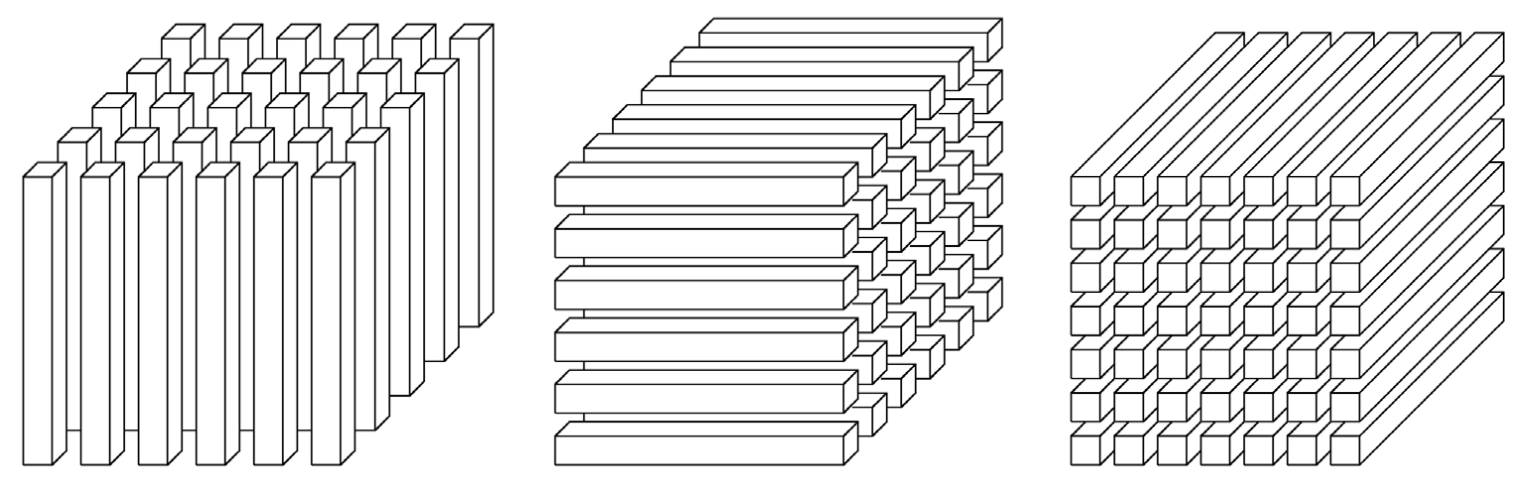
\includegraphics[scale=0.2]{images/fibers.png}
  \caption{De mode-1, mode-2 en mode-3 vezels van een 3D-tensor. Bron: Kolda en Bader \cite{ref:kolda}.}
\label{fig:fibers}
\end{figure}

Als men de mode-n vezels terug samen zet als een reeks kolommen in een matrix, bekomt men de mode-n \textit{matricisatie} van de tensor \cite{ref:kolda}. De volgorde waarin de vectoren in de matrix geordend worden, is niet van belang, zolang ze consistent is. We zullen dit opnieuw illustreren met een voorbeeld, gebaseerd op Kolda en Bader \cite{ref:kolda}. Stel we hebben een 3D-tensor $X \in \mathbb{R}^{4 \times 3 \times 2}$ waarvan de twee ``lagen'' (nu $X_1$ en $X_2$ genoemd), bepaald door de derde index, de volgende waarden bevatten:
\[
X_1 = \begin{bmatrix}
1 & 5 & 9 \\
2 & 6 & 10 \\
3 & 7 & 11 \\
4 & 8 & 12 \\
\end{bmatrix}
\quad
X_2 = \begin{bmatrix}
13 & 17 & 21 \\
14 & 18 & 22 \\
15 & 19 & 23 \\
16 & 20 & 24 \\
\end{bmatrix}
\]
\newpage
Dan zijn de verschillende mode-n matricisaties $X_{(n)}$:
\[
X_{(1)} = \begin{bmatrix}
1 & 5 & 9  & 13 & 17 & 21 \\
2 & 6 & 10 & 14 & 18 & 22 \\
3 & 7 & 11 & 15 & 19 & 23 \\
4 & 8 & 12 & 16 & 20 & 24 \\
\end{bmatrix}
\quad
X_{(2)} = \begin{bmatrix}
1 & 2  & 3  & 4  & 13 & 14 & 15 & 16 \\
5 & 6  & 7  & 8  & 17 & 18 & 19 & 20 \\
9 & 10 & 11 & 12 & 21 & 22 & 23 & 24 \\
\end{bmatrix}
\]
\[
X_{(3)} = \begin{bmatrix}
1  & 2  & 3  & 4  & 5  & 6  & 7  & 8  & 9  & 10 & 11 & 12 \\
13 & 14 & 15 & 16 & 17 & 18 & 19 & 20 & 21 & 22 & 23 & 24 \\
\end{bmatrix}
\]

Nu kunnen we ten slotte het tensor-matrix mode-n product defini\"eren. Wanneer men het mode-n product neemt van een tensor $X$ en een matrix $U$ (genoteerd als $X \times_n U$), komt dit simpelweg neer op het transformeren van alle mode-n vezels van $X$ door ze langs links te vermenigvuldigen met $U$. Formeel uitgedrukt, in functie van matricisaties en het matrix-product:
\[
Y = X \times_n U \Leftrightarrow Y_{(n)} = U X_{(n)}
\]
We zullen deze operatie zowel gebruiken om de Tucker-decompositie (later in dit hoofdstuk) en de tensor-train-decompositie (hoofdstuk \ref{hoofdstuk:hervorming}) te beschrijven.

\subsection{Singulierewaardenontbinding}

Een belangrijke matrixontbinding uit de lineaire algebra is de singulierewaardenontbinding, ook bekend als de SVD (\textit{singular value decomposition}) \cite{ref:svd}. Hierbij schrijven we de matrix $A \in \mathbb{R}^{m \times n}$ uit als het product $A = U \Sigma V^T$ waarbij $U \in \mathbb{R}^{m \times m}$ en $V \in \mathbb{R}^{n \times n}$ orthogonale matrices zijn en $\Sigma \in \mathbb{R}^{m \times n}$ een positieve diagonaalmatrix is. De kolommen van $U$ en $V$ noemen we respectievelijk de linker- en rechter-singuliere vectoren van $A$ en de diagonaalelementen van $\Sigma$ vormen de singuliere waarden van $A$ (deze staan ook gerangschikt van groot naar klein op de diagonaal).\\

Wanneer men alleen de eerste $k$ kolommen van $U$ en $V$ en de eerste $k$ diagonaalelementen van $\Sigma$ beschouwt, bekomt men de afgeknotte SVD $A_k = U_k \Sigma_k V_k^T$. Een interessante eigenschap hiervan is dat $A_k$ de beste rang-k benadering is van $A$ op vlak van Frobenius-norm. Men kan dit ook op een andere manier interpreteren: als de kolommen van $A$ een verzameling vectoren voorstellen, vormen de eerste $k$ linker-singuliere vectoren de beste $k$-dimensionale basis voor deze vectoren. Namelijk, als men de originele vectoren benadert door ze te orthogonaal projecteren op deze deelruimte, is de som van de kwadraten van de fouten op elke vector minimaal. Als men de rijen van de matrix als vectoren beschouwt, geldt hetzelfde maar dan voor de rechter-singuliere vectoren.

\subsection{Tucker-decompositie}

Een belangrijke decompositie voor tensoren is de Tucker-decompositie \cite{ref:tucker}. Hierbij wordt een tensor $A \in \mathbb{R}^{n_1 \times n_2 \times \dots \times n_d}$ met $d$ modes voorgesteld door een kerntensor $B \in \mathbb{R}^{r_1 \times r_2 \times \dots \times r_d}$ en $d$ factormatrices $U_1 \in \mathbb{R}^{n_1 \times r_1}$, $U_2 \in \mathbb{R}^{n_2 \times r_2}$, $\dots$, $U_d \in \mathbb{R}^{n_d \times r_d}$. Het verband tussen de originele tensor en de decompositie kan simpelweg gedefinieerd worden aan de hand van het mode-n product:
\[
A = B \times_1 U_1 \times_2 U_2 \times_3 \dots \times_d U_d
\]
We noemen $(r_1, \dots, r_d)$ de multilineaire rang van $B$ (later meestal de compressierang genoemd) en bijgevolg ook $A$. Stel dat we een tensor $A$ hebben met \'e\'en of meerdere modes $i$ waarvoor geldt $\text{rank}(A_{(i)}) > r_i$, dan kunnen we nog steeds een Tucker-decompositie gebruiken om $A$ benaderend voor te stellen met een (hopelijk kleine) fout, zoals we bij matrices deden met de afgeknotte SVD. Op deze manier kan men tensoren met een arbitrair aantal modes lossy comprimeren.\\

In tegenstelling tot bij matrices, is er helaas geen gekend algoritme om voor een bepaalde tensor $A$ en compressierang $(r_1, \dots, r_d)$ de optimale factormatrices $U_1, \dots, U_d$ te berekenen (als men het verschil op vlak van Frobeniusnorm probeert te minimaliseren). Er bestaat wel een iteratief algoritme, genaamd HOOI \cite{ref:kolda}, dat een lokaal optimum berekent, maar dit is te traag voor praktische doeleinden en is vooral nuttig als referentie bij het onderzoeken van de effici\"entie van niet-iteratieve algoritmen.

\subsection{T-HOSVD}

Vanwege de effectiviteit van de afgeknotte SVD bij het comprimeren van matrices, is het logisch om deze ook proberen te gebruiken voor hoger-dimensionale tensoren. Dit is wat men doet bij de T-HOSVD-procedure \cite{ref:kolda}: voor elke mode $i$ nemen we de eerste $r_i$ linker-singuliere vectoren van $A_{(i)}$ als factormatrix $U_i$. Daarna berekenen we de kerntensor $B$ door de vezels van $A$ langs elke mode orthogonaal te projecteren op de deelruimte bepaald door de corresponderende factormatrix:
\[
B = A \times_1 U_1^T \times_2 U_2^T \times_3 \dots \times_d U_d^T
\]

\subsection{ST-HOSVD}

Een andere manier om een Tucker-decompositie van een tensor te berekenen, ook gebaseerd op de SVD, is met de ST-HOSVD \cite{ref:st_hosvd}. Concreet verloopt deze procedure als volgt:\\

\begin{algorithm}[H]
\KwData{$A, (r_1, \dots, r_d)$}
\KwResult{$B$, $(U_1, \dots, U_d)$}
$B := A$\\
\For{$i = 1, ..., d$}{
$U_i := $ de eerste $r_i$ linker-singuliere vectoren van $B_{(i)}$\\
$B := B \times_i U_i^T$\\
}
\end{algorithm}

Analoog aan de T-HOSVD, wordt voor elke mode de afgeknotte SVD over de vezels langs die mode berekend en gebruikt als factormatrix. Het grote verschil is dat deze procedure sequentieel is: na het bepalen van een factormatrix, wordt deze meteen toegepast voordat de volgende modes verwerkt worden. Dit geeft de ST-HOSVD enkele voordelen:

\begin{itemize}
\item De sequenti\"ele uitvoeringstijd voor lage compressierangen ligt veel lager, omdat de tensor $B$ significant verkleind wordt doorheen het algoritme. Men kan de verschillende modes wel niet meer in parallel verwerken.
\item De benaderingsfout ligt in de praktijk bijna altijd lager dan bij de T-HOSVD \cite{ref:st_hosvd}.
\item In plaats van de multilineaire rang vast te leggen, kan men een doelfout $\epsilon$ geven als invoer, wat praktischer is in het geval van compressie. Bij de T-HOSVD kan men de doelfout per mode $\epsilon_i$ dan proberen te te verdelen volgens $\epsilon_i^2 = \frac{\epsilon^2}{d}$. In mode $i$ wordt $r_i$ zo gekozen zodat de som van de kwadraten van de weggelaten singuliere waarden uit de afgeknotte SVD kleiner dan of gelijk is aan $\epsilon_i^2$. Aangezien de rang per mode echter gekozen moet worden op discrete wijze, zal er altijd een marge zijn tussen de toegevoegde fout en $\epsilon_i^2$. Omdat de ST-HOSVD sequentieel werkt, kan men dit compenseren door $\epsilon_i$ zowel te laten afhangen van $\epsilon$, het aantal nog te verwerken modes en de fouten toegevoegd in eerdere modes. Op deze manier kan de ST-HOSVD een gegeven doelfout beter benaderen dan de T-HOSVD.
\end{itemize}

Vanwege deze voordelen zullen we voor het berekenen van Tucker-decomposities (en later ook \textit{tensor trains}) gebruik maken van de ST-HOSVD. Omdat dit algoritme sequentieel werkt, moeten we wel letten op de volgorde waarin de modes verwerkt worden. Wanneer de grootste compressie eerst gebeurd, is de kerntensor meteen sterk verkleind en kunnen de volgende modes sneller verwerkt worden, zodat de uitvoeringstijd daalt.